\begin{frame}
		\frametitle{From STL To Voxels}
		\begin{minipage}{0.85\textwidth}
			\begin{itemize}
			\item Used Common Versatile Multi-purpose Library for C++ (CVMLCPP)
			\item Takes .stl file and returns a binary file with the given voxel size
			\item Wrote script to read binary file and output it as ascii.vtk
			\end{itemize}
			\only<1>{			
			\centering
			\begin{figure}
			
\includegraphics[scale=0.15]{Pictures/STLToVoxels/Star_STL.png}
			\end{figure}
			}
			\only<2>{
			\centering
			\begin{figure}
			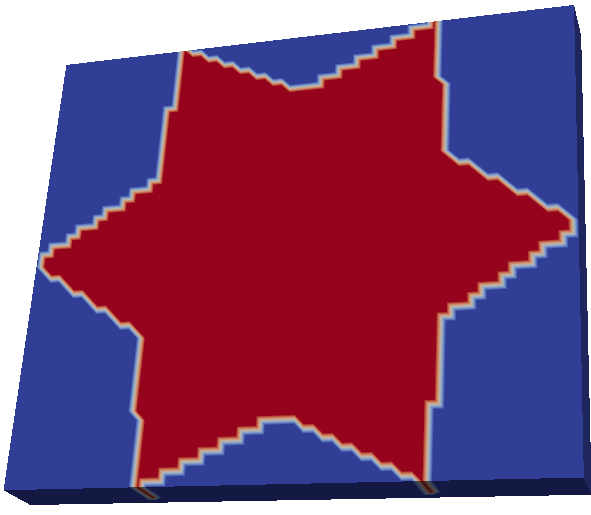
\includegraphics[scale=0.15]{Pictures/STLToVoxels/Star_VTK_Trans.png}
			\end{figure}
			}
			\only<3>{
			\centering
			\begin{figure}
			
\includegraphics[scale=0.15]{Pictures/STLToVoxels/Star_STL.png}
			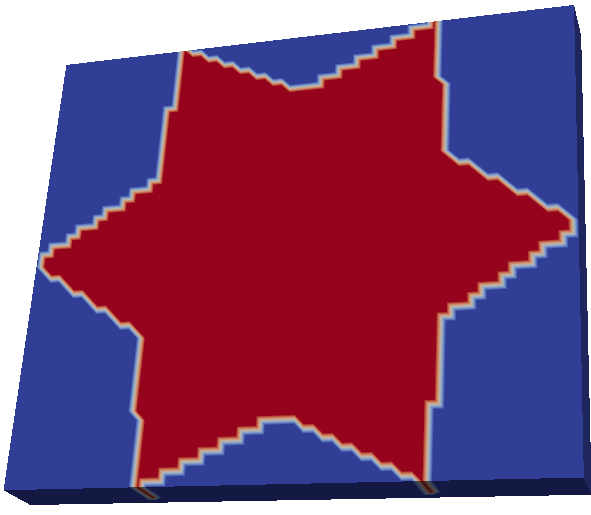
\includegraphics[scale=0.15]{Pictures/STLToVoxels/Star_VTK_Trans.png}
			\end{figure}
			}
		\end{minipage}
		\begin{minipage}{0.14\textwidth}
			\begin{figure}
				\scalebox{0.08}{
\includegraphics{Pictures/1CAD.pdf}}\\
				\scalebox{0.08}{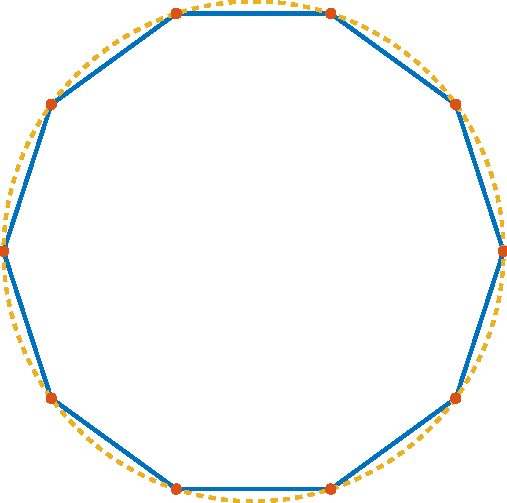
\includegraphics{Pictures/2STL.pdf}}\\
				\scalebox{0.08}{% This file was created by matlab2tikz.
% Minimal pgfplots version: 1.3
%
%The latest updates can be retrieved from
%  http://www.mathworks.com/matlabcentral/fileexchange/22022-matlab2tikz
%where you can also make suggestions and rate matlab2tikz.
%

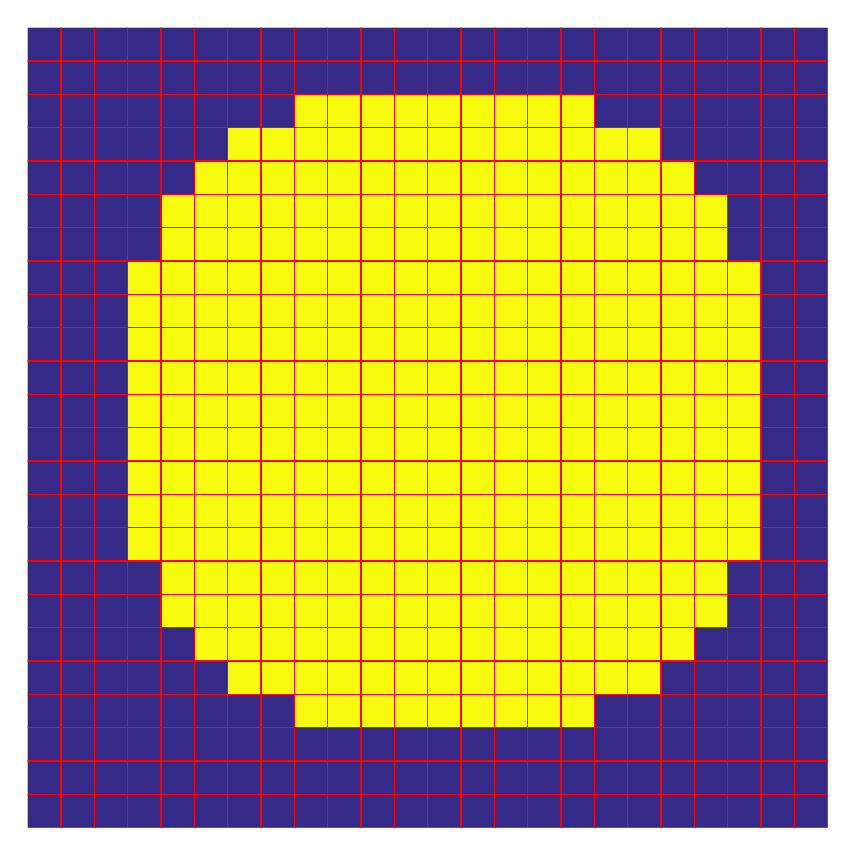
\begin{tikzpicture}[thin]

\begin{axis}[%
hide axis,
width=4in,
height=4in,
scale only axis,
view={0}{90},
]

\definecolor{edgecolor}{rgb}{1,0,0}

\addplot3[%
surf,
faceted color=black,
shader=flat corner,
draw=edgecolor,
colormap={mymap}{[1pt] rgb(0pt)=(0.2081,0.1663,0.5292); rgb(1pt)=(0.211624,0.189781,0.577676); rgb(2pt)=(0.212252,0.213771,0.626971); rgb(3pt)=(0.2081,0.2386,0.677086); rgb(4pt)=(0.195905,0.264457,0.7279); rgb(5pt)=(0.170729,0.291938,0.779248); rgb(6pt)=(0.125271,0.324243,0.830271); rgb(7pt)=(0.0591333,0.359833,0.868333); rgb(8pt)=(0.0116952,0.38751,0.881957); rgb(9pt)=(0.00595714,0.408614,0.882843); rgb(10pt)=(0.0165143,0.4266,0.878633); rgb(11pt)=(0.0328524,0.443043,0.871957); rgb(12pt)=(0.0498143,0.458571,0.864057); rgb(13pt)=(0.0629333,0.47369,0.855438); rgb(14pt)=(0.0722667,0.488667,0.8467); rgb(15pt)=(0.0779429,0.503986,0.838371); rgb(16pt)=(0.0793476,0.520024,0.831181); rgb(17pt)=(0.0749429,0.537543,0.826271); rgb(18pt)=(0.0640571,0.556986,0.823957); rgb(19pt)=(0.0487714,0.577224,0.822829); rgb(20pt)=(0.0343429,0.596581,0.819852); rgb(21pt)=(0.0265,0.6137,0.8135); rgb(22pt)=(0.0238905,0.628662,0.803762); rgb(23pt)=(0.0230905,0.641786,0.791267); rgb(24pt)=(0.0227714,0.653486,0.776757); rgb(25pt)=(0.0266619,0.664195,0.760719); rgb(26pt)=(0.0383714,0.674271,0.743552); rgb(27pt)=(0.0589714,0.683757,0.725386); rgb(28pt)=(0.0843,0.692833,0.706167); rgb(29pt)=(0.113295,0.7015,0.685857); rgb(30pt)=(0.145271,0.709757,0.664629); rgb(31pt)=(0.180133,0.717657,0.642433); rgb(32pt)=(0.217829,0.725043,0.619262); rgb(33pt)=(0.258643,0.731714,0.595429); rgb(34pt)=(0.302171,0.737605,0.571186); rgb(35pt)=(0.348167,0.742433,0.547267); rgb(36pt)=(0.395257,0.7459,0.524443); rgb(37pt)=(0.44201,0.748081,0.503314); rgb(38pt)=(0.487124,0.749062,0.483976); rgb(39pt)=(0.530029,0.749114,0.466114); rgb(40pt)=(0.570857,0.748519,0.44939); rgb(41pt)=(0.609852,0.747314,0.433686); rgb(42pt)=(0.6473,0.7456,0.4188); rgb(43pt)=(0.683419,0.743476,0.404433); rgb(44pt)=(0.71841,0.741133,0.390476); rgb(45pt)=(0.752486,0.7384,0.376814); rgb(46pt)=(0.785843,0.735567,0.363271); rgb(47pt)=(0.818505,0.732733,0.34979); rgb(48pt)=(0.850657,0.7299,0.336029); rgb(49pt)=(0.882433,0.727433,0.3217); rgb(50pt)=(0.913933,0.725786,0.306276); rgb(51pt)=(0.944957,0.726114,0.288643); rgb(52pt)=(0.973895,0.731395,0.266648); rgb(53pt)=(0.993771,0.745457,0.240348); rgb(54pt)=(0.999043,0.765314,0.216414); rgb(55pt)=(0.995533,0.786057,0.196652); rgb(56pt)=(0.988,0.8066,0.179367); rgb(57pt)=(0.978857,0.827143,0.163314); rgb(58pt)=(0.9697,0.848138,0.147452); rgb(59pt)=(0.962586,0.870514,0.1309); rgb(60pt)=(0.958871,0.8949,0.113243); rgb(61pt)=(0.959824,0.921833,0.0948381); rgb(62pt)=(0.9661,0.951443,0.0755333); rgb(63pt)=(0.9763,0.9831,0.0538)},
mesh/rows=25]
table[row sep=crcr,header=false] {%
%
-1.2	-1.2	0\\
-1.2	-1.1	0\\
-1.2	-1	0\\
-1.2	-0.9	0\\
-1.2	-0.8	0\\
-1.2	-0.7	0\\
-1.2	-0.6	0\\
-1.2	-0.5	0\\
-1.2	-0.4	0\\
-1.2	-0.3	0\\
-1.2	-0.2	0\\
-1.2	-0.0999999999999999	0\\
-1.2	0	0\\
-1.2	0.0999999999999999	0\\
-1.2	0.2	0\\
-1.2	0.3	0\\
-1.2	0.4	0\\
-1.2	0.5	0\\
-1.2	0.6	0\\
-1.2	0.7	0\\
-1.2	0.8	0\\
-1.2	0.9	0\\
-1.2	1	0\\
-1.2	1.1	0\\
-1.2	1.2	0\\
-1.1	-1.2	0\\
-1.1	-1.1	0\\
-1.1	-1	0\\
-1.1	-0.9	0\\
-1.1	-0.8	0\\
-1.1	-0.7	0\\
-1.1	-0.6	0\\
-1.1	-0.5	0\\
-1.1	-0.4	0\\
-1.1	-0.3	0\\
-1.1	-0.2	0\\
-1.1	-0.0999999999999999	0\\
-1.1	0	0\\
-1.1	0.0999999999999999	0\\
-1.1	0.2	0\\
-1.1	0.3	0\\
-1.1	0.4	0\\
-1.1	0.5	0\\
-1.1	0.6	0\\
-1.1	0.7	0\\
-1.1	0.8	0\\
-1.1	0.9	0\\
-1.1	1	0\\
-1.1	1.1	0\\
-1.1	1.2	0\\
-1	-1.2	0\\
-1	-1.1	0\\
-1	-1	0\\
-1	-0.9	0\\
-1	-0.8	0\\
-1	-0.7	0\\
-1	-0.6	0\\
-1	-0.5	0\\
-1	-0.4	0\\
-1	-0.3	0\\
-1	-0.2	0\\
-1	-0.0999999999999999	0\\
-1	0	0\\
-1	0.0999999999999999	0\\
-1	0.2	0\\
-1	0.3	0\\
-1	0.4	0\\
-1	0.5	0\\
-1	0.6	0\\
-1	0.7	0\\
-1	0.8	0\\
-1	0.9	0\\
-1	1	0\\
-1	1.1	0\\
-1	1.2	0\\
-0.9	-1.2	0\\
-0.9	-1.1	0\\
-0.9	-1	0\\
-0.9	-0.9	0\\
-0.9	-0.8	0\\
-0.9	-0.7	0\\
-0.9	-0.6	0\\
-0.9	-0.5	0\\
-0.9	-0.4	1\\
-0.9	-0.3	1\\
-0.9	-0.2	1\\
-0.9	-0.0999999999999999	1\\
-0.9	0	1\\
-0.9	0.0999999999999999	1\\
-0.9	0.2	1\\
-0.9	0.3	1\\
-0.9	0.4	1\\
-0.9	0.5	0\\
-0.9	0.6	0\\
-0.9	0.7	0\\
-0.9	0.8	0\\
-0.9	0.9	0\\
-0.9	1	0\\
-0.9	1.1	0\\
-0.9	1.2	0\\
-0.8	-1.2	0\\
-0.8	-1.1	0\\
-0.8	-1	0\\
-0.8	-0.9	0\\
-0.8	-0.8	0\\
-0.8	-0.7	0\\
-0.8	-0.6	1\\
-0.8	-0.5	1\\
-0.8	-0.4	1\\
-0.8	-0.3	1\\
-0.8	-0.2	1\\
-0.8	-0.0999999999999999	1\\
-0.8	0	1\\
-0.8	0.0999999999999999	1\\
-0.8	0.2	1\\
-0.8	0.3	1\\
-0.8	0.4	1\\
-0.8	0.5	1\\
-0.8	0.6	1\\
-0.8	0.7	0\\
-0.8	0.8	0\\
-0.8	0.9	0\\
-0.8	1	0\\
-0.8	1.1	0\\
-0.8	1.2	0\\
-0.7	-1.2	0\\
-0.7	-1.1	0\\
-0.7	-1	0\\
-0.7	-0.9	0\\
-0.7	-0.8	0\\
-0.7	-0.7	1\\
-0.7	-0.6	1\\
-0.7	-0.5	1\\
-0.7	-0.4	1\\
-0.7	-0.3	1\\
-0.7	-0.2	1\\
-0.7	-0.0999999999999999	1\\
-0.7	0	1\\
-0.7	0.0999999999999999	1\\
-0.7	0.2	1\\
-0.7	0.3	1\\
-0.7	0.4	1\\
-0.7	0.5	1\\
-0.7	0.6	1\\
-0.7	0.7	1\\
-0.7	0.8	0\\
-0.7	0.9	0\\
-0.7	1	0\\
-0.7	1.1	0\\
-0.7	1.2	0\\
-0.6	-1.2	0\\
-0.6	-1.1	0\\
-0.6	-1	0\\
-0.6	-0.9	0\\
-0.6	-0.8	1\\
-0.6	-0.7	1\\
-0.6	-0.6	1\\
-0.6	-0.5	1\\
-0.6	-0.4	1\\
-0.6	-0.3	1\\
-0.6	-0.2	1\\
-0.6	-0.0999999999999999	1\\
-0.6	0	1\\
-0.6	0.0999999999999999	1\\
-0.6	0.2	1\\
-0.6	0.3	1\\
-0.6	0.4	1\\
-0.6	0.5	1\\
-0.6	0.6	1\\
-0.6	0.7	1\\
-0.6	0.8	1\\
-0.6	0.9	0\\
-0.6	1	0\\
-0.6	1.1	0\\
-0.6	1.2	0\\
-0.5	-1.2	0\\
-0.5	-1.1	0\\
-0.5	-1	0\\
-0.5	-0.9	0\\
-0.5	-0.8	1\\
-0.5	-0.7	1\\
-0.5	-0.6	1\\
-0.5	-0.5	1\\
-0.5	-0.4	1\\
-0.5	-0.3	1\\
-0.5	-0.2	1\\
-0.5	-0.0999999999999999	1\\
-0.5	0	1\\
-0.5	0.0999999999999999	1\\
-0.5	0.2	1\\
-0.5	0.3	1\\
-0.5	0.4	1\\
-0.5	0.5	1\\
-0.5	0.6	1\\
-0.5	0.7	1\\
-0.5	0.8	1\\
-0.5	0.9	0\\
-0.5	1	0\\
-0.5	1.1	0\\
-0.5	1.2	0\\
-0.4	-1.2	0\\
-0.4	-1.1	0\\
-0.4	-1	0\\
-0.4	-0.9	1\\
-0.4	-0.8	1\\
-0.4	-0.7	1\\
-0.4	-0.6	1\\
-0.4	-0.5	1\\
-0.4	-0.4	1\\
-0.4	-0.3	1\\
-0.4	-0.2	1\\
-0.4	-0.0999999999999999	1\\
-0.4	0	1\\
-0.4	0.0999999999999999	1\\
-0.4	0.2	1\\
-0.4	0.3	1\\
-0.4	0.4	1\\
-0.4	0.5	1\\
-0.4	0.6	1\\
-0.4	0.7	1\\
-0.4	0.8	1\\
-0.4	0.9	1\\
-0.4	1	0\\
-0.4	1.1	0\\
-0.4	1.2	0\\
-0.3	-1.2	0\\
-0.3	-1.1	0\\
-0.3	-1	0\\
-0.3	-0.9	1\\
-0.3	-0.8	1\\
-0.3	-0.7	1\\
-0.3	-0.6	1\\
-0.3	-0.5	1\\
-0.3	-0.4	1\\
-0.3	-0.3	1\\
-0.3	-0.2	1\\
-0.3	-0.0999999999999999	1\\
-0.3	0	1\\
-0.3	0.0999999999999999	1\\
-0.3	0.2	1\\
-0.3	0.3	1\\
-0.3	0.4	1\\
-0.3	0.5	1\\
-0.3	0.6	1\\
-0.3	0.7	1\\
-0.3	0.8	1\\
-0.3	0.9	1\\
-0.3	1	0\\
-0.3	1.1	0\\
-0.3	1.2	0\\
-0.2	-1.2	0\\
-0.2	-1.1	0\\
-0.2	-1	0\\
-0.2	-0.9	1\\
-0.2	-0.8	1\\
-0.2	-0.7	1\\
-0.2	-0.6	1\\
-0.2	-0.5	1\\
-0.2	-0.4	1\\
-0.2	-0.3	1\\
-0.2	-0.2	1\\
-0.2	-0.0999999999999999	1\\
-0.2	0	1\\
-0.2	0.0999999999999999	1\\
-0.2	0.2	1\\
-0.2	0.3	1\\
-0.2	0.4	1\\
-0.2	0.5	1\\
-0.2	0.6	1\\
-0.2	0.7	1\\
-0.2	0.8	1\\
-0.2	0.9	1\\
-0.2	1	0\\
-0.2	1.1	0\\
-0.2	1.2	0\\
-0.0999999999999999	-1.2	0\\
-0.0999999999999999	-1.1	0\\
-0.0999999999999999	-1	0\\
-0.0999999999999999	-0.9	1\\
-0.0999999999999999	-0.8	1\\
-0.0999999999999999	-0.7	1\\
-0.0999999999999999	-0.6	1\\
-0.0999999999999999	-0.5	1\\
-0.0999999999999999	-0.4	1\\
-0.0999999999999999	-0.3	1\\
-0.0999999999999999	-0.2	1\\
-0.0999999999999999	-0.0999999999999999	1\\
-0.0999999999999999	0	1\\
-0.0999999999999999	0.0999999999999999	1\\
-0.0999999999999999	0.2	1\\
-0.0999999999999999	0.3	1\\
-0.0999999999999999	0.4	1\\
-0.0999999999999999	0.5	1\\
-0.0999999999999999	0.6	1\\
-0.0999999999999999	0.7	1\\
-0.0999999999999999	0.8	1\\
-0.0999999999999999	0.9	1\\
-0.0999999999999999	1	0\\
-0.0999999999999999	1.1	0\\
-0.0999999999999999	1.2	0\\
0	-1.2	0\\
0	-1.1	0\\
0	-1	0\\
0	-0.9	1\\
0	-0.8	1\\
0	-0.7	1\\
0	-0.6	1\\
0	-0.5	1\\
0	-0.4	1\\
0	-0.3	1\\
0	-0.2	1\\
0	-0.0999999999999999	1\\
0	0	1\\
0	0.0999999999999999	1\\
0	0.2	1\\
0	0.3	1\\
0	0.4	1\\
0	0.5	1\\
0	0.6	1\\
0	0.7	1\\
0	0.8	1\\
0	0.9	1\\
0	1	0\\
0	1.1	0\\
0	1.2	0\\
0.0999999999999999	-1.2	0\\
0.0999999999999999	-1.1	0\\
0.0999999999999999	-1	0\\
0.0999999999999999	-0.9	1\\
0.0999999999999999	-0.8	1\\
0.0999999999999999	-0.7	1\\
0.0999999999999999	-0.6	1\\
0.0999999999999999	-0.5	1\\
0.0999999999999999	-0.4	1\\
0.0999999999999999	-0.3	1\\
0.0999999999999999	-0.2	1\\
0.0999999999999999	-0.0999999999999999	1\\
0.0999999999999999	0	1\\
0.0999999999999999	0.0999999999999999	1\\
0.0999999999999999	0.2	1\\
0.0999999999999999	0.3	1\\
0.0999999999999999	0.4	1\\
0.0999999999999999	0.5	1\\
0.0999999999999999	0.6	1\\
0.0999999999999999	0.7	1\\
0.0999999999999999	0.8	1\\
0.0999999999999999	0.9	1\\
0.0999999999999999	1	0\\
0.0999999999999999	1.1	0\\
0.0999999999999999	1.2	0\\
0.2	-1.2	0\\
0.2	-1.1	0\\
0.2	-1	0\\
0.2	-0.9	1\\
0.2	-0.8	1\\
0.2	-0.7	1\\
0.2	-0.6	1\\
0.2	-0.5	1\\
0.2	-0.4	1\\
0.2	-0.3	1\\
0.2	-0.2	1\\
0.2	-0.0999999999999999	1\\
0.2	0	1\\
0.2	0.0999999999999999	1\\
0.2	0.2	1\\
0.2	0.3	1\\
0.2	0.4	1\\
0.2	0.5	1\\
0.2	0.6	1\\
0.2	0.7	1\\
0.2	0.8	1\\
0.2	0.9	1\\
0.2	1	0\\
0.2	1.1	0\\
0.2	1.2	0\\
0.3	-1.2	0\\
0.3	-1.1	0\\
0.3	-1	0\\
0.3	-0.9	1\\
0.3	-0.8	1\\
0.3	-0.7	1\\
0.3	-0.6	1\\
0.3	-0.5	1\\
0.3	-0.4	1\\
0.3	-0.3	1\\
0.3	-0.2	1\\
0.3	-0.0999999999999999	1\\
0.3	0	1\\
0.3	0.0999999999999999	1\\
0.3	0.2	1\\
0.3	0.3	1\\
0.3	0.4	1\\
0.3	0.5	1\\
0.3	0.6	1\\
0.3	0.7	1\\
0.3	0.8	1\\
0.3	0.9	1\\
0.3	1	0\\
0.3	1.1	0\\
0.3	1.2	0\\
0.4	-1.2	0\\
0.4	-1.1	0\\
0.4	-1	0\\
0.4	-0.9	1\\
0.4	-0.8	1\\
0.4	-0.7	1\\
0.4	-0.6	1\\
0.4	-0.5	1\\
0.4	-0.4	1\\
0.4	-0.3	1\\
0.4	-0.2	1\\
0.4	-0.0999999999999999	1\\
0.4	0	1\\
0.4	0.0999999999999999	1\\
0.4	0.2	1\\
0.4	0.3	1\\
0.4	0.4	1\\
0.4	0.5	1\\
0.4	0.6	1\\
0.4	0.7	1\\
0.4	0.8	1\\
0.4	0.9	1\\
0.4	1	0\\
0.4	1.1	0\\
0.4	1.2	0\\
0.5	-1.2	0\\
0.5	-1.1	0\\
0.5	-1	0\\
0.5	-0.9	0\\
0.5	-0.8	1\\
0.5	-0.7	1\\
0.5	-0.6	1\\
0.5	-0.5	1\\
0.5	-0.4	1\\
0.5	-0.3	1\\
0.5	-0.2	1\\
0.5	-0.0999999999999999	1\\
0.5	0	1\\
0.5	0.0999999999999999	1\\
0.5	0.2	1\\
0.5	0.3	1\\
0.5	0.4	1\\
0.5	0.5	1\\
0.5	0.6	1\\
0.5	0.7	1\\
0.5	0.8	1\\
0.5	0.9	0\\
0.5	1	0\\
0.5	1.1	0\\
0.5	1.2	0\\
0.6	-1.2	0\\
0.6	-1.1	0\\
0.6	-1	0\\
0.6	-0.9	0\\
0.6	-0.8	1\\
0.6	-0.7	1\\
0.6	-0.6	1\\
0.6	-0.5	1\\
0.6	-0.4	1\\
0.6	-0.3	1\\
0.6	-0.2	1\\
0.6	-0.0999999999999999	1\\
0.6	0	1\\
0.6	0.0999999999999999	1\\
0.6	0.2	1\\
0.6	0.3	1\\
0.6	0.4	1\\
0.6	0.5	1\\
0.6	0.6	1\\
0.6	0.7	1\\
0.6	0.8	1\\
0.6	0.9	0\\
0.6	1	0\\
0.6	1.1	0\\
0.6	1.2	0\\
0.7	-1.2	0\\
0.7	-1.1	0\\
0.7	-1	0\\
0.7	-0.9	0\\
0.7	-0.8	0\\
0.7	-0.7	1\\
0.7	-0.6	1\\
0.7	-0.5	1\\
0.7	-0.4	1\\
0.7	-0.3	1\\
0.7	-0.2	1\\
0.7	-0.0999999999999999	1\\
0.7	0	1\\
0.7	0.0999999999999999	1\\
0.7	0.2	1\\
0.7	0.3	1\\
0.7	0.4	1\\
0.7	0.5	1\\
0.7	0.6	1\\
0.7	0.7	1\\
0.7	0.8	0\\
0.7	0.9	0\\
0.7	1	0\\
0.7	1.1	0\\
0.7	1.2	0\\
0.8	-1.2	0\\
0.8	-1.1	0\\
0.8	-1	0\\
0.8	-0.9	0\\
0.8	-0.8	0\\
0.8	-0.7	0\\
0.8	-0.6	1\\
0.8	-0.5	1\\
0.8	-0.4	1\\
0.8	-0.3	1\\
0.8	-0.2	1\\
0.8	-0.0999999999999999	1\\
0.8	0	1\\
0.8	0.0999999999999999	1\\
0.8	0.2	1\\
0.8	0.3	1\\
0.8	0.4	1\\
0.8	0.5	1\\
0.8	0.6	1\\
0.8	0.7	0\\
0.8	0.8	0\\
0.8	0.9	0\\
0.8	1	0\\
0.8	1.1	0\\
0.8	1.2	0\\
0.9	-1.2	0\\
0.9	-1.1	0\\
0.9	-1	0\\
0.9	-0.9	0\\
0.9	-0.8	0\\
0.9	-0.7	0\\
0.9	-0.6	0\\
0.9	-0.5	0\\
0.9	-0.4	1\\
0.9	-0.3	1\\
0.9	-0.2	1\\
0.9	-0.0999999999999999	1\\
0.9	0	1\\
0.9	0.0999999999999999	1\\
0.9	0.2	1\\
0.9	0.3	1\\
0.9	0.4	1\\
0.9	0.5	0\\
0.9	0.6	0\\
0.9	0.7	0\\
0.9	0.8	0\\
0.9	0.9	0\\
0.9	1	0\\
0.9	1.1	0\\
0.9	1.2	0\\
1	-1.2	0\\
1	-1.1	0\\
1	-1	0\\
1	-0.9	0\\
1	-0.8	0\\
1	-0.7	0\\
1	-0.6	0\\
1	-0.5	0\\
1	-0.4	0\\
1	-0.3	0\\
1	-0.2	0\\
1	-0.0999999999999999	0\\
1	0	0\\
1	0.0999999999999999	0\\
1	0.2	0\\
1	0.3	0\\
1	0.4	0\\
1	0.5	0\\
1	0.6	0\\
1	0.7	0\\
1	0.8	0\\
1	0.9	0\\
1	1	0\\
1	1.1	0\\
1	1.2	0\\
1.1	-1.2	0\\
1.1	-1.1	0\\
1.1	-1	0\\
1.1	-0.9	0\\
1.1	-0.8	0\\
1.1	-0.7	0\\
1.1	-0.6	0\\
1.1	-0.5	0\\
1.1	-0.4	0\\
1.1	-0.3	0\\
1.1	-0.2	0\\
1.1	-0.0999999999999999	0\\
1.1	0	0\\
1.1	0.0999999999999999	0\\
1.1	0.2	0\\
1.1	0.3	0\\
1.1	0.4	0\\
1.1	0.5	0\\
1.1	0.6	0\\
1.1	0.7	0\\
1.1	0.8	0\\
1.1	0.9	0\\
1.1	1	0\\
1.1	1.1	0\\
1.1	1.2	0\\
1.2	-1.2	0\\
1.2	-1.1	0\\
1.2	-1	0\\
1.2	-0.9	0\\
1.2	-0.8	0\\
1.2	-0.7	0\\
1.2	-0.6	0\\
1.2	-0.5	0\\
1.2	-0.4	0\\
1.2	-0.3	0\\
1.2	-0.2	0\\
1.2	-0.0999999999999999	0\\
1.2	0	0\\
1.2	0.0999999999999999	0\\
1.2	0.2	0\\
1.2	0.3	0\\
1.2	0.4	0\\
1.2	0.5	0\\
1.2	0.6	0\\
1.2	0.7	0\\
1.2	0.8	0\\
1.2	0.9	0\\
1.2	1	0\\
1.2	1.1	0\\
1.2	1.2	0\\
};
\end{axis}
\end{tikzpicture}%
%\end{document}}\\
				\scalebox{0.08}{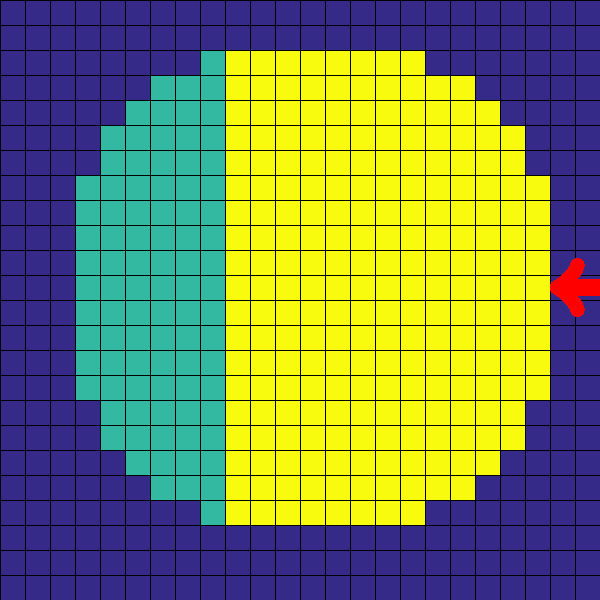
\includegraphics{Pictures/4TPD.pdf}}\\
				\scalebox{0.08}{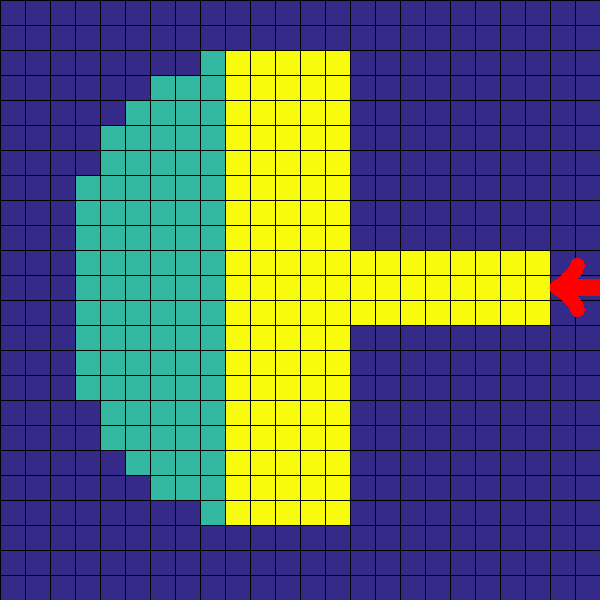
\includegraphics{Pictures/5TOPOPT.pdf}}\\
				\scalebox{0.08}{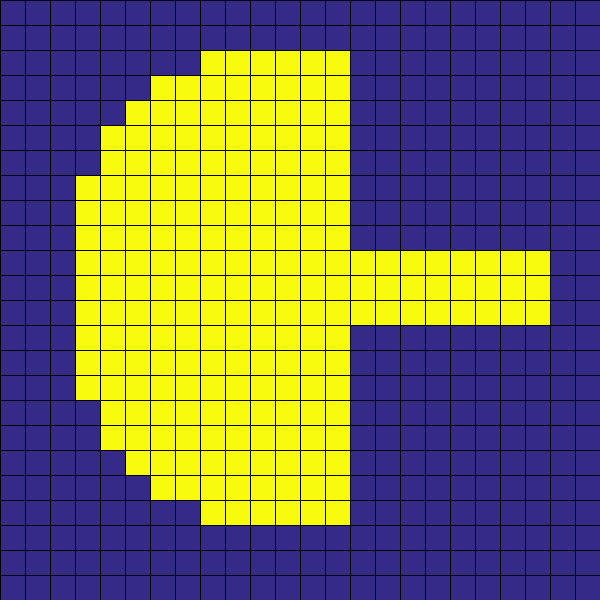
\includegraphics{Pictures/6TOPYOUT.pdf}}\\
				\scalebox{0.08}{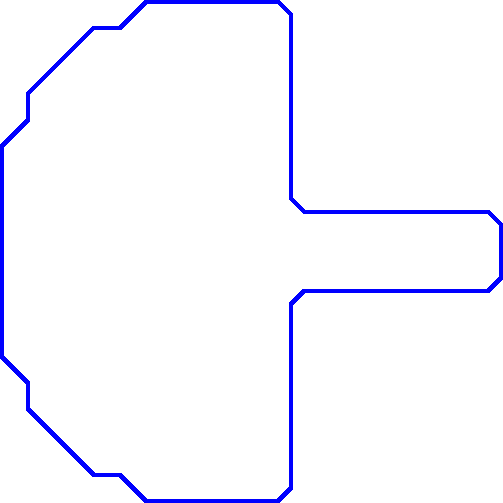
\includegraphics{Pictures/7MC.pdf}}
			\end{figure}
		\end{minipage}
\end{frame}